\documentclass[12pt]{book}
\usepackage{graphicx}
\graphicspath{{./images/}}
\usepackage[a4paper, left=2cm, right=2cm]{geometry}
\title{مبانی آنالیز ریاضی}
\author{علی سینا سلطانی و ؟؟}
\date{}

\usepackage{amsmath}
\usepackage{amssymb, amsthm}
\usepackage{centernot}
\usepackage{fancyhdr}
\usepackage{xepersian}

\linespread{1.25}
\pagestyle{fancy}
\settextfont{0 Nazanin}
%\newfontfamily\myfont{IranNastaliq}
%\setlength{\abovedisplayskip}{-15pt}
%\setlength{\belowdisplayskip}{0pt}
%\setlength{\abovedisplayshortskip}{0pt}
%\setlength{\belowdisplayshortskip}{0pt}

\fancyhf{}
\fancyhead[ER]{\thepage \quad مبانی آنالیز ریاضی}
\fancyhead[OL]{فضای متریک \quad \thepage}

\newtheorem{thm}{\textbf{قضیه}}
\newtheorem{df}[thm]{\textbf{تعریف}}
\newtheorem{col}[thm]{\textbf{نتیجه}}
\newtheorem{ex}[thm]{\textbf{مثال}}
\begin{document}
%	\maketitle
%	\topskip0pt
%	\vspace*{\fill}
%	\begin{center}
%		\myfont{
%		\Huge{تقدیم به خورشیدی که با غروبش،‌\\تاریکی شب را با من آشنا کرد.}
%		}
%	\end{center}
%	\vspace*{\fill}
	\chapter{فضای متریک}\label{CH1: Metric Space}
	فرض کنیم میدونیم متر به چه درد میخوره
	\begin{df}\label{Def1: Metric Space}
		مجموعه ای مانند \( X \) یک \textbf{فضای متریک} است اگر تابعی مانند \( d:X \times X \to \mathbb{R} \) که تابع فاصله نامیده می‌شود وجود داشته باشد،\, ‌به طوری که:
		\begin{enumerate}
			\item[الف)] 
			فاصله هر دو نقطه متمایز \( X \)،‌\, یک عدد حقیقی مثبت باشد و فاصله هر عضو با خودش صفر باشد.
			\begin{align}
				\forall p,q \in X,\quad p \centernot = q,\quad d(p,\ q) \geq 0 \quad and \quad d(p,\ p) = 0
			\end{align}
			\item[ب)]
			برای هر دو عضو دلخواه \( p \) و  \( q \) در  \( X \)،\, فاصله‌ی \( p \) تا \( q \)،‌\, برابر با فاصله \( q \) تا \( p \) باشد.
		\begin{align}
			\forall p\ ,q \in X, \quad d(p,\ q) = d(q,\ p)
		\end{align}
		\item[ج)]
		تابع  \( d \) خاصیت مثلثی داشته باشد یعنی برای هر سه عضو دلخواه \( p \) و \( q \) و \( r \) در \( X \)، فاصله \( p \) تا \( q \) کمتر مساوی مجموع فاصله \( p \) تا \( r \) و \( q \) تا \( r \) است.
		\begin{align}
			\forall p\ ,q\ ,r\ \in X, \quad d(p,\ q) \leq d(p,\ r)\ + \ d(q,\ r)
		\end{align}
		\end{enumerate}
	به هر عضو از فضای متریک  \( X \)،\, نقطه گفته می‌شود.
	\end{df}
	\pagebreak
	\begin{df}\label{Def2: Intervals}
		منظور از بازه‌ی باز \( (a,\, b) \)، مجموعه‌ی همه‌ی اعداد حقیقی مانند \( x \) است به طوری که:‌\quad 
		\( a <\, x\, <\, b \)
		\begin{align}
			(a,\, b) = \{x \in \mathbb{R} \mid a <\, x <\, b\}
		\end{align}
		منظور از بازه‌ی بسته‌ی \( (a,\, b) \)، مجموعه‌ی همه‌ی اعداد حقیقی مانند \( x \) است به طوری که:‌\quad 
		\( a \leq \, x\, \leq \, b \)
		\begin{align}
			[a,\, b] = \{x \in \mathbb{R} \mid a \leq\, x \leq\, b\}
		\end{align}
	به همین روش بازه های نیم بسته \( [a, b) \) و \( [a, b) \) را هم تعریف می کنیم:
		\begin{align}
			(a, b] = \{x \in \mathbb{R} \mid a <\, x \leq\, b\} \quad 
			[a, b) = \{x \in \mathbb{R} \mid a \leq\, x <‌\, b \}
		\end{align}
	\end{df}

	\begin{df}\label{Def3: k-cell}
		فرض کنید برای هر \(i = 1,\cdots, k\)،‌ \( [a_i, b_i] \) بازه‌ی بسته‌ای در \( \mathbb{R} \) باشد.\\
		در نتیجه
		\( [a_1,\, b_1] \times \cdots \times [a_k,\, b_k] \subset \mathbb{R}^k \).\\
		مجموعه‌ی همه نقاط 
		\(\ x = (x_1,\,\cdots,\, x_k) \in \mathbb{R}^k \)
		به طوری که
		\( \forall i = 1,\, \cdots ,\, k \ \ \  a_i \leq\, x_i \leq\, b_i \)
		یک سلول یا حجره \(k\)-بعدی نامیده می‌شود.\\
		\begin{align}
			K-cell = \{ x = (x_1,\ \ldots,\ x_k) \in \mathbb{R}^k\ \mid\ \forall i = 1,\ \ldots,\ k \ \ \ a_i<\ x_i<\ b_i \}
		\end{align}
		بنابراین هر سلول 1-بعدی،\ ‌یک بازه و هر سلول 2-بعدی،\  یک مستطیل است و...
	\end{df}
	
	\noindent
	حالا که توانستیم تعریف مناسبی برای متر،‌\ فضای متریک و فاصله‌ی دو نقطه پیدا کنیم،‌\ برای بهتر شناختن فضای متریک،\ لازم داریم تا نقطه‌هایی که از یک نقطه مشخص،\ به فاصله‌ای مشخص قرار دارند را شناسایی کنیم.\\
	در واقع می‌خواهیم همسایه‌های یک نقطه در فضای متریک را پیدا کنیم.\ به همین منظور در ادامه با مفهوم همسایگی آشنا می‌شویم.
	\begin{df}\label{Def4: Neighborhood}
		اگر \( (X,\ d) \) یک فضای متریک باشد،‌\ یک همسایگی به مرکز \( x \in X \) و شعاع \( r>0 \) را مجموعه همه‌ی نقاطی مانند \( y \in X \) تعریف می‌کنیم،\ به طوری که: 
		\( d(x,\ y)\ <\ r \) و آن را با 
		\( N_r(x) \) نشان می‌دهیم.
		\begin{align}
			N_r(x) = \{ y \in X \mid d(x,\ y) <\ r \}
		\end{align}
	\end{df}

	\begin{df}\label{Def5: Convex Combination}
		اگر 
		\( x \) و \( y \) 
		دو نقطه در فضای متریک
		 \( \mathbb{R}^2 \) 
		 با متر متعارف باشند،\  ترکیب محدب 
		\( x \) و \( y \)
		،\ ‌ ترکیب خطی این دو نقطه به صورت 
		\( \alpha x +‌\beta y \)
		 است،\ ‌ به طوری که ضرایب 
		 \( \alpha \) و \( \beta \)
		  اعداد حقیقی نامنفی باشند و 
		 \( \alpha +‌ \beta = 1 \).\\
		 به طور کلی،\ ترکیب محدب نقاط 
		 \( x_1,\ \ldots,\ x_n \in \mathbb{R}^k  \)
		 ،‌\ ترکیب خطی
		  \( \sum_{i = 0}^{n} \alpha_i x_i \)
		   است که در آن ضرایب 
		   \( \alpha_i \)
		    اعداد حقیقی نامنفی هستند و 
		    \( \alpha_1 +\ \ldots +\ \alpha_n = 1 \)\ . \\
		 توجه کنید که حاصل هر ترکیب محدب از دو نقطه،\ یک نقطه دیگر خواهد بود.
	\end{df}

	\begin{df}\label{Def6: Convex Set}
		مجموعه‌ی \( X \) محدب است،‌\ اگر و تنها اگر به ازای هر دو نقطه \( x \)،‌\ ترکیب محدب این دو نقطه در \( x \) موجود باشد. \ یعنی:
		\begin{align}
			\forall x, y \in X,\  \forall \alpha, \beta \in [0, 1] \ \  s.t \ \ \alpha +‌ \beta = 1, \ \  \alpha x +‌ \beta y \in X
		\end{align}
		اگر ضرایب \( \alpha \) و \( \beta \) را به ترتیب \( t \) و \( t-1 \) در نظر بگیریم،\ خواهیم داشت:
		\begin{align}
			\forall x, y \in X,\ \ \forall t \in [0,1], \ \ tx +‌(1-t)y \in X
		\end{align}
	\end{df}
	
	\noindent 
	در عبارت (1.7) قرار می‌دهیم
	  \( t = 0 \) 
	  و ترکیب محدب دو نقطه‌ی \( x \) و \( y \) را به دست می‌آوریم:
	   \(0x +‌ (1-0)y = y \) \\
	همینطور برای \( t = 1 \) داریم:
	 \( x +‌(1-1)y = x \)\ . \\
	بنابراین هرچه مقدار \( t \) از 0 به 1 نزدیک‌تر شود، \ نقطه‌ی حاصل از ترکیب محدب از \( y \) به سمت \( x \) حرکت می‌کند.\\
	پس مجموعه‌ی همه ترکیب‌های محدب \( x \) و \( y \) برای مقادیر \( t \) از 0 تا 1،\ تشکیل خطی را می‌دهد که \( x \) را به \( y \) وصل می‌کند و می‌توان نتیجه گرفت:
	\begin{col}\label{Col7: Geometric Consept of Convex Set}
		مجموعه \( X \) محدب است،\ اگر و تنها اگر برای هر دو نقطه‌ی \( x, y \in X\)،\ خطی که \( x \) و \( y \)  را به هم وصل می‌کند هم در \( X \) موجود باشد.
	\end{col}

	\begin{ex}
		دو نقطه \( (1, 2) \) و \( (3 ,4) \) را در نظر بگیرید.
		با انتخاب  مقادیر
		\( t \)
		در بازه 0 و 1، همینطور که در شکل \ref{convex_ex_1} می‌توان دید،‌\ نقطه‌های حاصل از ترکیب محدب دو نقطه،\ خط واصل این دو نقطه را تشکیل می‌دهند.
		\begin{figure}[h]
			\centering
			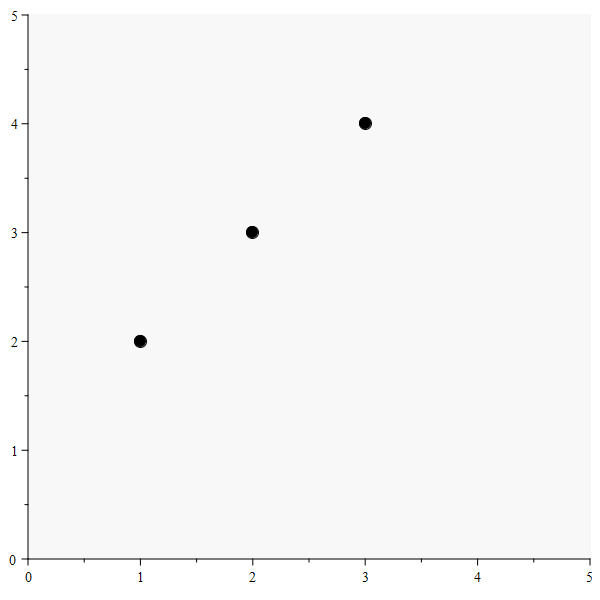
\includegraphics[width=0.25\textwidth]{convex_line_1}
			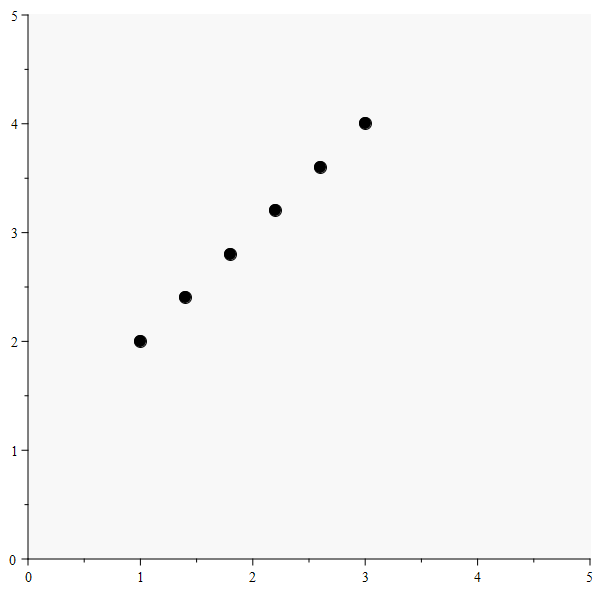
\includegraphics[width=0.25\textwidth]{convex_line_2}
			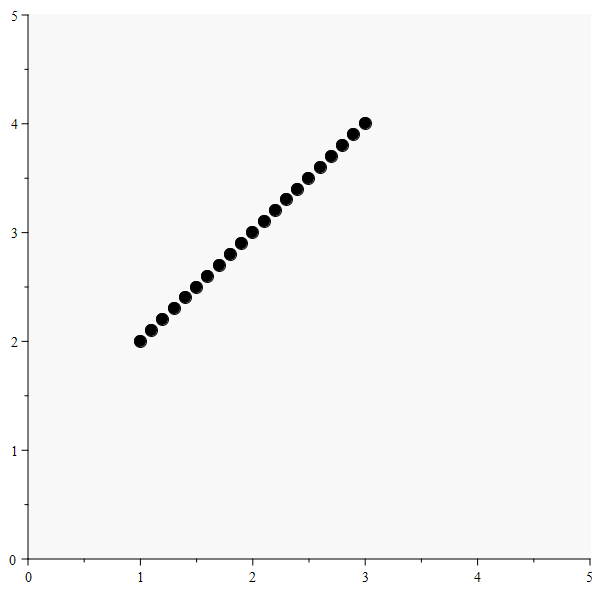
\includegraphics[width=0.25\textwidth]{convex_line_3}
			\caption{‌مجموعه‌ی همه‌ی ترکیب‌های محدب دو نقطه،\ خط واصل دو نقطه را تشکیل می‌دهد. }
			\label{convex_ex_1}
		\end{figure}
	\end{ex}
	\pagebreak
	\begin{ex}
		شکل‌های زیر هم مثال‌هایی از مجموعه‌های محدب	هستند.
		\begin{figure}[h]
			\centering
			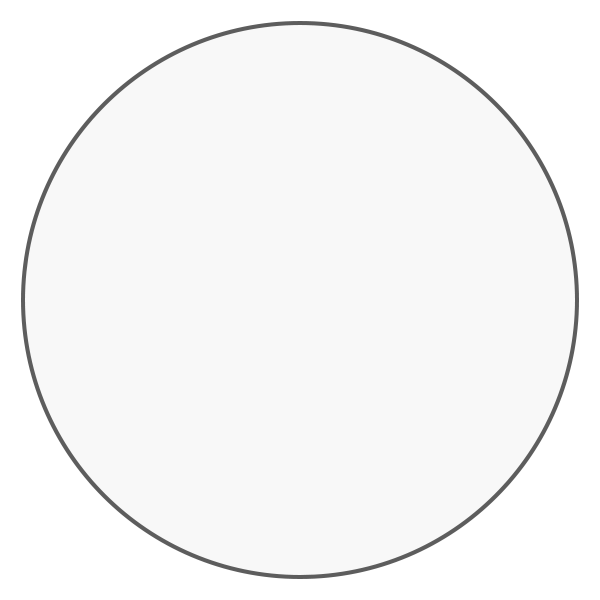
\includegraphics[width=0.25\textwidth]{convex_circle}
			
\includegraphics[width=0.25\textwidth]{convex_square}
			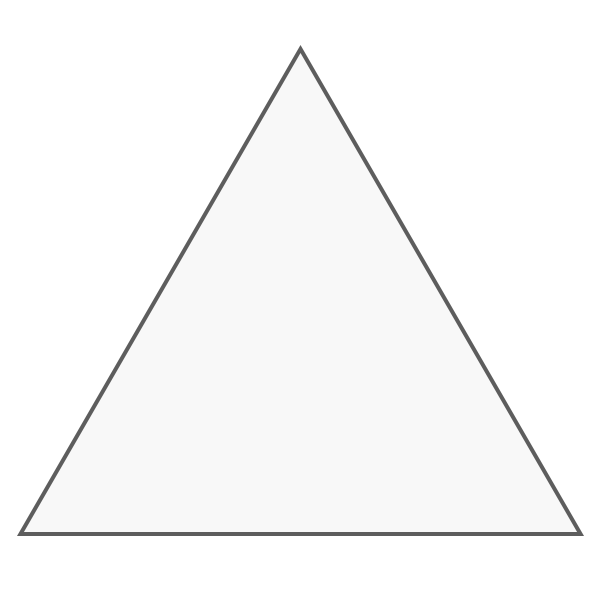
\includegraphics[width=0.25\textwidth]{convex_triangle}
			\caption{‌}
			\label{convex_ex_2}
		\end{figure}
		\begin{figure}[h]
			\centering
			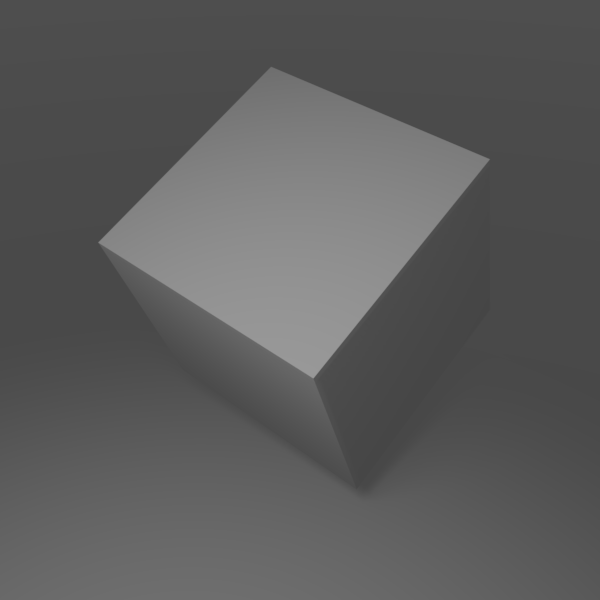
\includegraphics[width=0.25\textwidth]{convex_cube}
			
\includegraphics[width=0.25\textwidth]{convex_tetrahedron}
			
\includegraphics[width=0.25\textwidth]{convex_octahedron}
			\caption{‌}
			\label{convex_ex_3}
		\end{figure}
	\end{ex}
	
%	\begin{ex}
	%	با توجه به تعریف محدب بودن یک مجموعه،‌\ محدب بودن یا %نبودن مجموعه‌های زیر را مشخص کنید.
%	\end{ex}
\pagebreak
	\begin{ex}
		اثبات کنید همسایگی‌ها مجموعه‌های محدب هستند.\\
		\vspace{-.7cm}
		\begin{proof}
			فرض کنید \( (X, d) \) یک فضای متریک باشد.\\
			طبق تعریف مجموعه‌های محدب،\ باید نشان دهیم ترکیب محدب هر دو عضو از یک همسایگی به مرکز \( x \in X \) و شعاع \( r>0 \)\ ،\ \\در خود همسایگی وجود دارد.\\
			یعنی اگر \( y \) و \( z \) دو عضور از همسایگی \( N_{r}(x) \) باشند،\ ترکیب محدب آن‌ها
			\( \lambda y + (1-\lambda) z  \)
			در همسایگی \( N_{r}(x) \) وجود دارد.
			\begin{align*}
				&N_{r}(x)\ is\ convex\ if:\\
				&\forall y,z \in N_{r}(x) ,\ (\lambda y + (1-\lambda) z) \in N_{r}(x)\\
				&Assume\ x, y \in N_{r}(x) \implies |y - x|<r\ \  and\ \  |z - x|<r\\
				&|\lambda y +‌(1-\lambda)z - x| = |\lambda y +‌(1-\lambda)z - x + \lambda x - \lambda x|\\
				&\leq |\lambda (y - x) + (1 - \lambda) (z - x)|\\
				&\leq |\lambda (y - x)| + |(1 - \lambda) (z - x)|\\
				&\leq \lambda|y - x| + (1 - \lambda)|z - x|\\
				&\leq \lambda r + (1 - \lambda)r\\
				&= r\\
				&Therefore: \forall y,z \in N_{r}(x), (\lambda y +‌(1-\lambda)z - x) \in N_{r}(x)
			\end{align*}
		\end{proof}
	\end{ex}
%	\pagebreak
%	\begin{flushright}
%		\myfont{
%			\textbf{
%				آفتابا\, غروب\, تو\, دیدم\\
%				خیز\, کم‌کم\, از\, خواب\, و\, سحر کن\\
	%			سرد\, بوده\, است\, جان\, من\, اینجا\\
		%		گرم\, کن\, جان\, من\, گرمتر\, کن\\
%			}
%		}
%	\end{flushright}
\end{document}